\subsection{Experimental Scenarios}

\textcolor{red}{Contents: i) objectives of test; ii) test scenario description: table of setting parameters for A2G; mobility of ue, number ue, number of test repetition (for statistically correct); iii) how to measure the evaluation metrics}
\subsubsection{Experiment Objectives}

The first objective is to evaluate the effect of UE/UAV altitude on the generated radio measurements. A higher aerial UE may have a higher probability of LOS connection to several gNBs, which can improve the serving-link received power but can also increase interference from neighboring cells. Therefore, altitude is expected to affect RSRP and SINR in different ways.

The second objective is to evaluate mobility and handover behavior. The simulator records the serving BS, neighboring-cell RSRP values, UE velocity, and handover indicators. These outputs make it possible to identify when the serving BS changes, where handover events occur along the trajectory, and whether the number of handovers changes across altitude ranges.

The third objective is to evaluate protocol-level handover delay under selected delay and loss settings. This part uses handover-emulation logs to measure completion time, timeout behavior, and failure cases. The purpose is not to merge radio measurement and protocol delay into one metric, but to compare the radio-level trigger behavior with the protocol-level execution behavior.

\subsubsection{Altitude-Range Design}

The altitude cases are grouped by height intervals rather than by a single fixed UAV height. This design follows the height regimes used by the propagation models in Chapter 2 and Chapter 3. In the 3GPP UMa model, low-height terrestrial UE modelling is used for \(1.5\le h_{\mathrm{UE}}\le22.5\) m. The height-correction term in the LOS-probability expression becomes active above 13 m. For aerial vehicles, 3GPP TR 36.777 extends the UMa model to UMa-AV conditions for \(22.5<h_{\mathrm{UE}}\le300\) m, with the implemented aerial NLOS expression used up to 100 m and a LOS-dominant high-altitude branch above 100 m \cite{3gpp_38901,3gpp_36777}.

\begin{table}[H]
\centering
\caption{Altitude ranges used for A2G radio-measurement experiments}
\small
\renewcommand{\arraystretch}{1.12}
\begin{tabularx}{\textwidth}{p{2.2cm}p{3.2cm}X}
\toprule
Range & Height interval & Model interpretation\\
\midrule
H0 & \(1.5\le h_{\mathrm{UE}}\le13\) m & Ground or low terrestrial UE range under the UMa model.\\
\addlinespace[2pt]
H1 & \(13<h_{\mathrm{UE}}\le22.5\) m & Elevated terrestrial or low-height UE range under the UMa model.\\
\addlinespace[2pt]
H2 & \(22.5<h_{\mathrm{UE}}\le100\) m & Low-to-medium aerial UE range under the UMa-AV model.\\
\addlinespace[2pt]
H3 & \(100<h_{\mathrm{UE}}\le300\) m & High aerial UE range under the UMa-AV model.\\
\bottomrule
\end{tabularx}
\renewcommand{\arraystretch}{1.0}
\label{tab:altitude-ranges-a2g}
\end{table}

The main A2G comparison uses H2 and H3, because these ranges represent aerial UE operation. H0 is kept as the terrestrial baseline, and H1 is kept as a transition range between ordinary ground-level operation and aerial operation. When detailed plots are produced, one representative height may be selected from each range for time-series visualization, while repeated runs within the same range are used for aggregate statistics.

\subsubsection{Scenario Description}

\begin{table}[H]
\centering
\caption{Experimental scenario groups}
\small
\begin{tabularx}{\textwidth}{p{1.7cm}X X}
\toprule
Scenario & Description & Purpose\\
\midrule
S1 & Baseline terrestrial and low-height UE scenario using H0 and H1. & Provide a reference for comparing aerial UE radio behavior.\\
\addlinespace[2pt]
S2 & A2G scenario with different altitude ranges using H2 and H3. & Analyze the impact of UAV altitude on RSRP, SINR, shadow fading, serving-cell changes, and handover indicators.\\
\addlinespace[2pt]
S3 & A2G scenario with different handover-delay or transport-delay settings. & Analyze the impact of delay on handover completion time, timeout cases, and failure behavior.\\
\bottomrule
\end{tabularx}
\label{tab:experimental-scenario-groups}
\end{table}

The radio simulation settings are kept fixed across altitude scenarios except for UE height. This makes the altitude effect easier to interpret because the carrier frequency, gNB transmit power, antenna gains, bandwidth, noise figure, handover margin, and mobility model remain unchanged.

\begin{table}[H]
\centering
\caption{Main simulation settings for A2G experiments}
\small
\begin{tabularx}{\textwidth}{p{4.0cm}p{3.4cm}X}
\toprule
Parameter & Value & Role in the experiment\\
\midrule
Carrier frequency & 2 GHz & Used in path-loss calculation\\
gNB transmit power & 46 dBm & Downlink link-budget parameter\\
gNB antenna gain / UE antenna gain & 2 dB / 0 dB & Used in received-power calculation\\
gNB antenna height & 25 m & Ground gNB height\\
UE height & Ranges H0--H3 & Main variable in altitude scenarios\\
Bandwidth / UE noise figure & 10 MHz / 9 dB & Used in thermal-noise calculation\\
Handover margin & 3 dB & RSRP-based serving-cell change condition\\
Mobility model & Manhattan mobility & UE moves along an urban road grid\\
UE speed & 20--60 km/h & Randomly assigned by the simulator\\
Simulation duration & 300 steps & One-second output interval\\
Number of UEs & 1 for trace plots; multiple UEs for aggregate runs & Controls whether the result is trajectory-level or aggregate-level\\
Repetitions & 30 runs per scenario & Reduces randomness from mobility, LOS/NLOS sampling, and shadow fading\\
\bottomrule
\end{tabularx}
\label{tab:a2g-simulation-settings}
\end{table}

For statistically meaningful comparison, each scenario should be repeated with different random seeds or independently generated UE trajectories. In this thesis, 30 repetitions per scenario are planned as the default setting. If execution time is limited, at least 10 repetitions can be used for preliminary analysis, but final comparison should report the number of repetitions explicitly.

\subsubsection{Evaluation Metrics}

The radio-level metrics are extracted from the simulator CSV output. RSRP is used to evaluate serving-cell and neighboring-cell signal strength. SINR is used to evaluate link quality under interference and thermal noise. Shadow fading is used to observe slow large-scale signal variation. UE velocity is used to interpret how fast the radio condition changes along the trajectory. The serving BS index and handover flag are used to identify cell changes and handover events.

For each scenario, the evaluation includes both time-series and scenario-level statistics. Time-series plots show how RSRP, SINR, shadow fading, speed, and serving BS evolve along one representative UE trajectory. Scenario-level plots compare the distribution or average value of RSRP, SINR, and number of handovers across altitude ranges or delay settings. The handover-related metrics include the number of handovers, handover event time, source and target BS, success rate, failure rate, and successful-trial handover delay when protocol-level logs are available.

\subsection{Radio Measurement Results}

This subsection reports the radio measurements generated by the simulator. The main plotted metrics are RSRP, SINR, shadow fading, and UE velocity. These metrics are analyzed together because they describe different parts of the same radio condition. RSRP mainly represents the received strength of the serving or neighboring cell, SINR represents the useful-signal quality after interference and noise are considered, shadow fading represents slow random variation around the median path loss, and velocity explains how quickly the UE moves through changing radio conditions.

The result presentation should include the following figures after the official simulation runs are generated:

\begin{itemize}
    \item RSRP over time for representative altitude ranges;
    \item SINR over time for representative altitude ranges;
    \item shadow fading over time for the serving link;
    \item UE velocity over time;
    \item RSRP comparison across altitude ranges;
    \item SINR comparison across altitude ranges.
\end{itemize}

When the UE moves farther from the serving gNB, the received signal strength generally decreases, which leads to a lower RSRP. However, RSRP is not determined only by distance. The LOS/NLOS state and shadow fading can also change the received power, so the RSRP curve may fluctuate even when the UE trajectory is smooth.

SINR can vary differently from RSRP because it depends on the serving-cell received power, neighboring-cell interference, and thermal noise. In aerial scenarios, a higher UE altitude may increase LOS visibility to the serving gNB, but it may also increase visibility to neighboring gNBs. Therefore, an altitude range with stronger RSRP does not always produce better SINR. Near cell-edge regions, or when several neighboring gNBs are received strongly, SINR may decrease even if the serving-cell RSRP remains acceptable.

Shadow fading explains slow signal variation caused by environmental obstruction and large-scale propagation randomness. In the simulator, the shadow-fading value is cached per UE--gNB link and updated after a movement distance threshold. As a result, shadow fading changes more slowly than instantaneous geometry-based received power and can create signal fluctuation even when the UE movement does not change abruptly.

Velocity is included to support interpretation of the radio time series. A faster UE moves through serving-cell and neighboring-cell regions more quickly, so RSRP and SINR may change more rapidly and handover opportunities may appear closer together in time. The velocity curve is therefore useful when explaining whether radio-measurement changes are caused by propagation conditions alone or by rapid movement through the cellular layout.

\subsection{Handover Behavior Analysis}

The radio simulator identifies handover events from serving-BS changes. A handover indicator is recorded when the selected serving BS differs from the previous serving BS. This radio-level handover event should be interpreted as a serving-cell transition suggested by the measurement model, not as a completed protocol-level handover procedure.

The handover behavior should be evaluated using the following outputs:

\begin{itemize}
    \item serving BS over time;
    \item handover event timeline;
    \item number of handovers per altitude range;
    \item source and target BS for each handover event;
    \item UE position and speed at each handover event;
    \item comparison between handover count and altitude range.
\end{itemize}

Handover events are expected to occur mainly when the UE moves toward the boundary between two cells. In this region, the RSRP of a neighboring gNB may become higher than the RSRP of the current serving gNB by more than the configured handover margin. A higher speed can make these transitions occur over fewer simulation steps, while a higher altitude can change the number of visible candidate gNBs and the interference condition. Therefore, the handover analysis should be interpreted together with the RSRP, SINR, and velocity plots rather than from the handover count alone.

For protocol-level delay analysis, the handover-emulation results are evaluated separately using trial-summary and timer-event logs. The main metrics are success rate, failure rate, timeout cases, mean successful handover delay, median successful handover delay, and 95th-percentile successful handover delay. This separation preserves the distinction between a radio-level serving-cell change and the completion of the actual handover signaling procedure.

\subsection{Validation Scope}

The handover-delay results in this chapter are obtained from StormSim trial-summary CSV files and timer-event logs generated while StormSim interacts with the free5GC core network. The repository contains many development logs but no single clearly labeled complete factorial experiment. Two large Xn runs with a logged one-way delay parameter of 20 ms are used for the verified comparison. Because the \texttt{pdr} field is populated from \texttt{PacketLoss}, its values are interpreted as loss probabilities.

\begin{table}[H]
\centering
\caption{Verified handover summaries}
\begin{tabular}{lrrrrr}
\toprule
Run & Loss & Trials & Success & Failure & Rate\\
\midrule
1781614531 & 0.10 & 210 & 210 & 0 & 100.00\%\\
1781622441 & 0.50 & 195 & 171 & 24 & 87.69\%\\
\bottomrule
\end{tabular}
\end{table}

\textbf{TODO:} Confirm that these are official rather than debugging runs.

\begin{figure}[H]
\centering
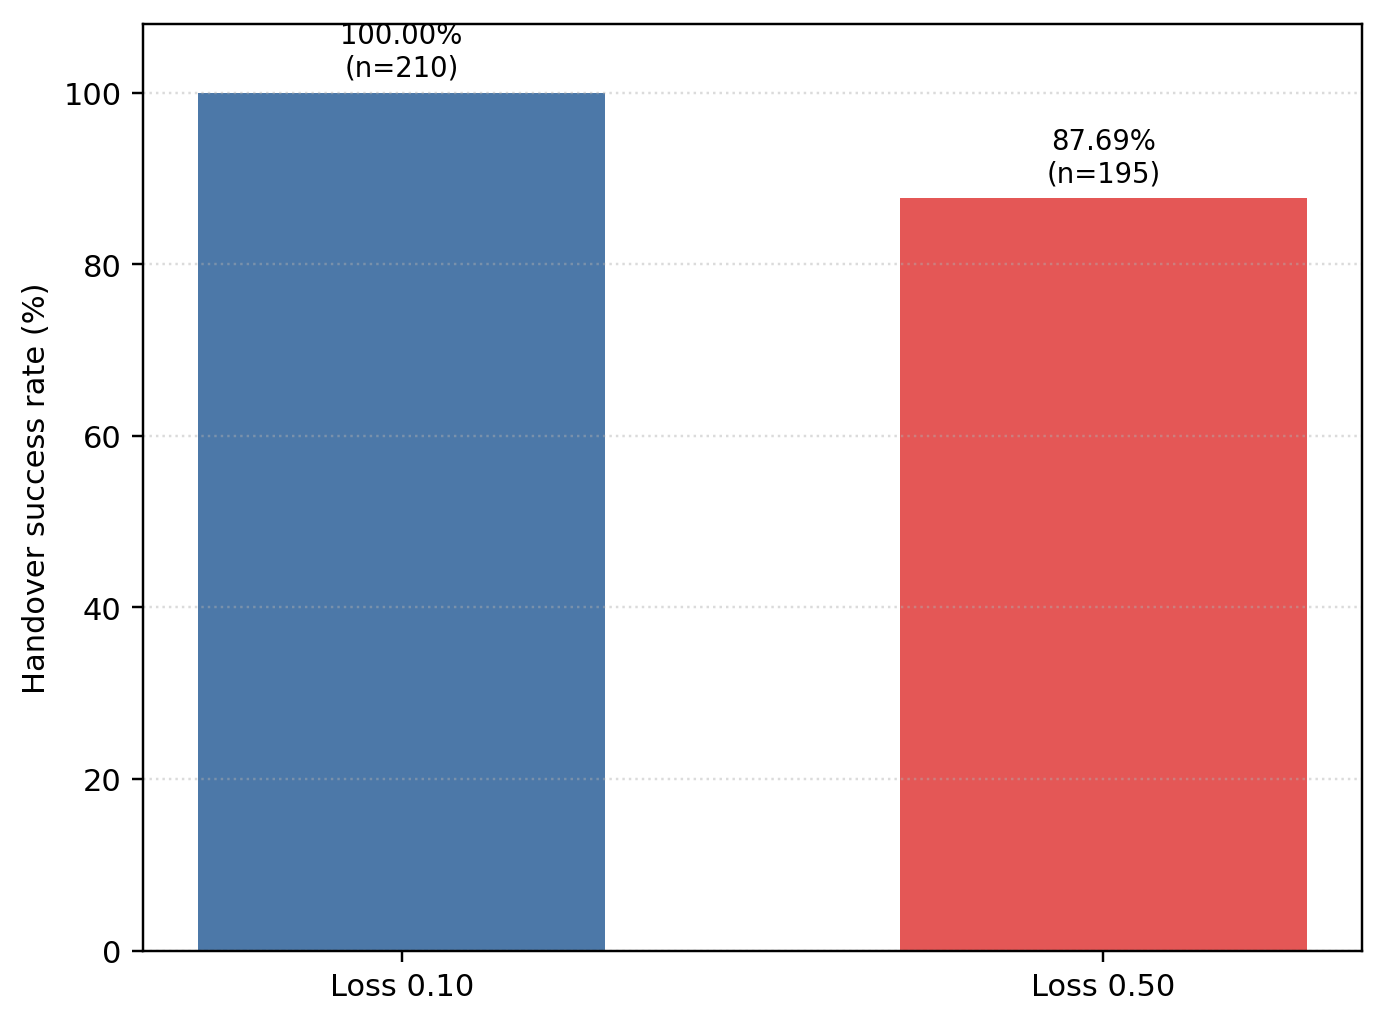
\includegraphics[width=0.82\textwidth]{Images/archived_ho_success_rate.png}
\caption{Handover success rate reproduced from the two archived trial-summary files}
\label{fig:archived-ho-success}
\end{figure}

Figure~\ref{fig:archived-ho-success} is descriptive rather than a controlled loss-response curve. The runs have different archived trial counts, and the exact source revision is unknown.

\subsection{Handover Success and Delay}

At loss 0.10, all 210 attempts succeeded. At loss 0.50, 171 of 195 succeeded; all 24 failures were labeled \texttt{Timeout}. The matching timer file contains 24 Xn preparation transport failures, 24 preparation timeouts, and 24 overall cancellations, associating these failures with unsuccessful Xn preparation.

\begin{figure}[H]
\centering
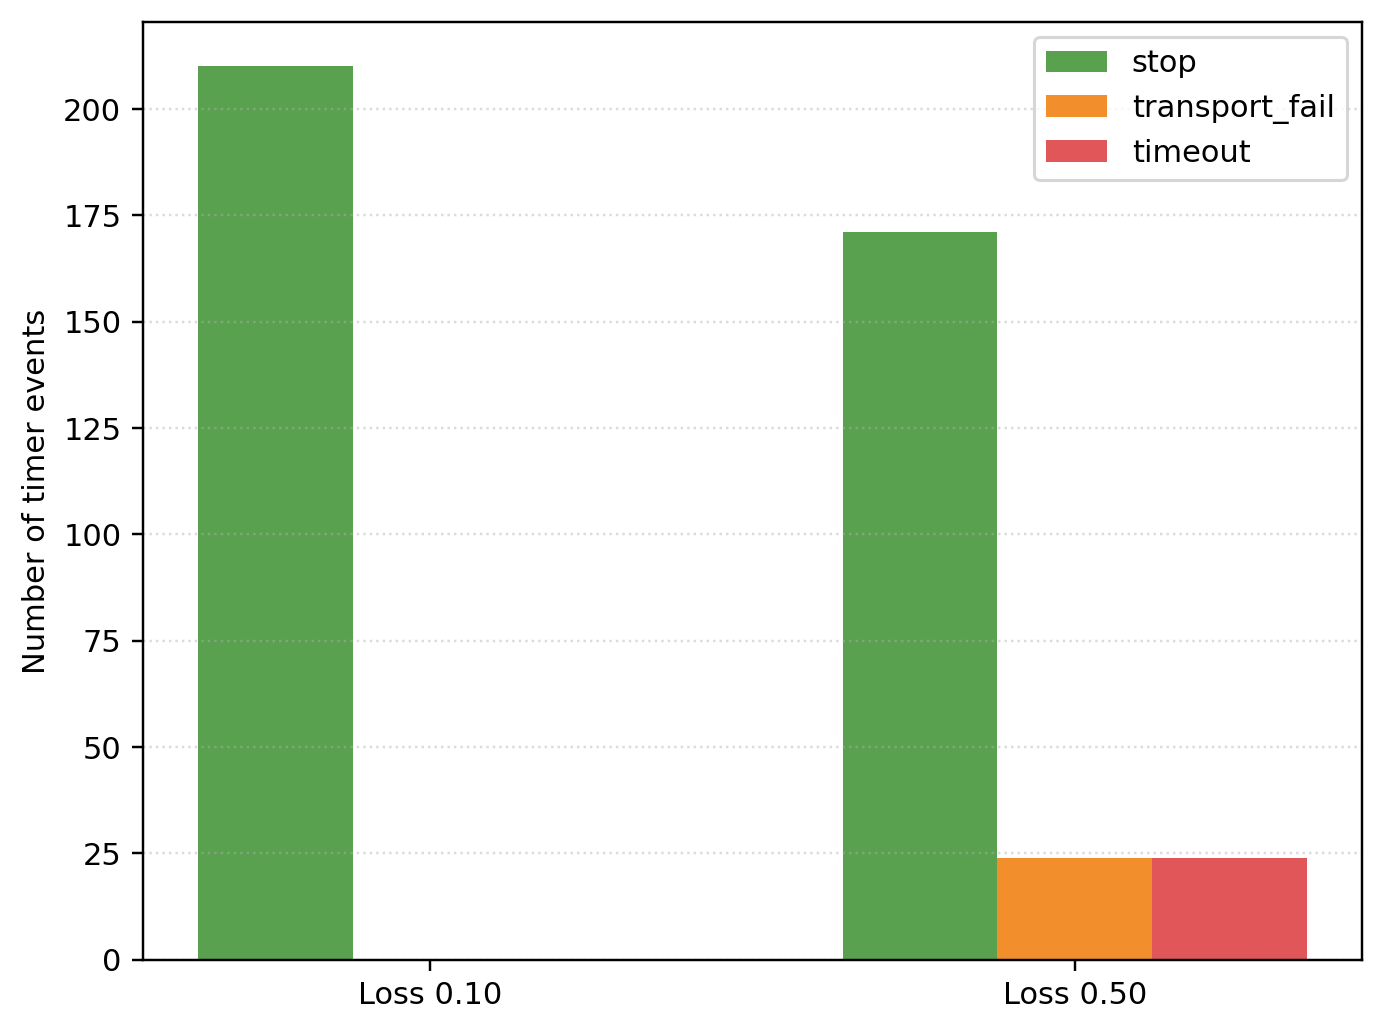
\includegraphics[width=0.82\textwidth]{Images/archived_xn_prep_outcomes.png}
\caption{TXnRELOCprep terminal and diagnostic events in the archived timer files}
\label{fig:archived-xn-prep}
\end{figure}

The \texttt{transport\_fail} and \texttt{timeout} bars at loss 0.50 describe the same 24 failed preparation lifecycles at different points: context forwarding first reports a transport failure, while the preparation timer is intentionally left active and later expires. They must not be added as 48 independent failed handovers.

\begin{table}[H]
\centering
\caption{Successful Xn handover delay}
\begin{tabular}{lrrr}
\toprule
Loss & Mean & Median & 95th percentile\\
\midrule
0.10 & 200.597 ms & 200.574 ms & 201.061 ms\\
0.50 & 200.627 ms & 200.628 ms & 201.062 ms\\
\bottomrule
\end{tabular}
\end{table}

Successful durations cluster around 200.6 ms because the scenario polls completion every 200 ms. The value is therefore quantized and is not a precise lower-layer latency measurement.

\begin{figure}[H]
\centering
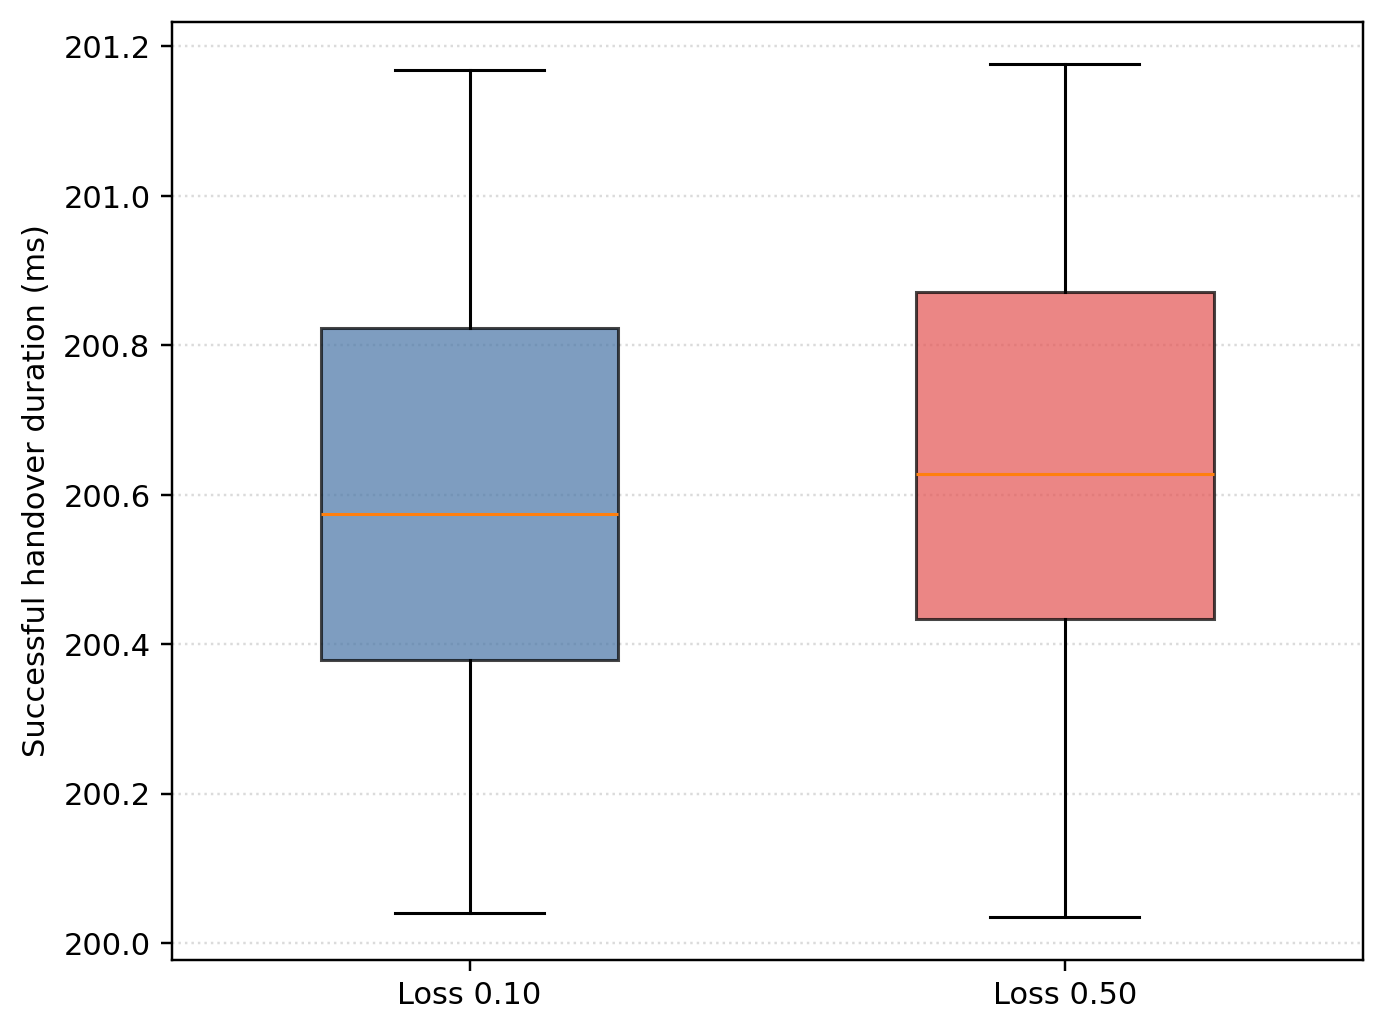
\includegraphics[width=0.82\textwidth]{Images/archived_ho_delay_boxplot.png}
\caption{Distribution of successful handover durations in the archived trial summaries}
\label{fig:archived-ho-delay}
\end{figure}

The narrow boxes in Fig.~\ref{fig:archived-ho-delay} do not demonstrate intrinsically low protocol jitter. They mainly show that the outer scenario observes completion at a 200 ms polling boundary.

\subsection{Timer Consistency and Missing Scenarios}

Raw timer coverage is incomplete. Run 1781614531 has 210 successful summaries but only 50 terminal T304 records, including one T304 timeout despite no failed trial. Trial summaries are therefore used as the authoritative overall outcome; T304 timeout rates are not reported.

The source supports several planned experiment outputs: loss--delay evaluation, a T304 breakpoint search, an RLF cascade, an Xn/N2 comparison, and beam-failure analysis. However, the repository does not contain a clearly labeled complete result set for all scenarios. RLF, beam, and N2 RTT fields are generally empty or zero.

There is also evidence that the archived logs were not generated by the exact current source state. The current Xn trigger sets the handover connection delay to T304 plus 500 ms, which should deliberately exceed T304, whereas archived successful records show T304 stopping after tens of milliseconds. The archived statistics are valid descriptions of those CSV files, but they cannot yet be claimed as reproducible results of the current executable revision.

\textbf{TODO:} Identify the archived source revision, then repeat the official timer campaign after fixing T304 and timer lifecycle coverage.

\subsection{Chapter Conclusion}

This chapter defined the experimental scenario groups for radio-measurement and handover-delay analysis. The altitude design follows the height regimes used by the UMa and UMa-AV propagation models, so the A2G experiments can compare terrestrial, transition, low-to-medium aerial, and high-aerial UE behavior. The chapter also described the planned radio-measurement plots and the metrics used to interpret RSRP, SINR, shadow fading, velocity, serving-cell changes, and handover events. The verified archived Xn runs demonstrate measurement-driven handover execution and show reduced success under higher signaling loss, while the delay results reveal polling quantization and timer-telemetry limitations. The next chapter summarizes the thesis, states the main limitations, and outlines future work.
